\section{Variable Temperature SRFs}
%==================================
\label{app:Tset}
This appendix contains the comparisons of the low spectral resolution digitized SRFs at low (-10\textdegree{}C), nominal (20\textdegree{}C), and high (50\textdegree{}C) baseplate temperature for nominal bias voltage (Vnom) from the ATMS PFM Calibration Data Book\cite{ATMS_PFM_CalLog}. The digitizations were performed by Lynn Chidester of the Space Dynamics Laboratory (SDL) at Utah State University. Included in the SRF plots are the ``boxcar'' SRF, based on the table \ref{tab:atms_fo_sb_and_df} data, and a representative brightness temperature spectrum.

Shown alongside each SRF comparison are the brightness temperature differences for the SRFs with respect to the boxcar response. MonoRTM \cite{Clough_2005} was used to compute the top-of-atmosphere brightness temperatures for the ECMWF83 profile data set \cite{ECMWF_profile_set2,Matricardi_ECMWF564} at the frequencies of the SRFs. These monochromatic brightness temperatures were then integrated over frequency to provide the channel brightness temperatures.

\newpage

% Note: the "[H]" placement option is allowed due to the use of the float package
%       in the preamble. I did this to avoid the
%        ! LaTeX Error: Too many unprocessed floats.
%       error due to the large number of figures.
\begin{figure}[H]
  \centering
  \begin{tabular}{c c c}
    \textsf{\textbf{(a)} SRFs} &
    \textsf{\textbf{(b)} $\Delta T_B$ $(\epsilon_s = 1.0)$} &
    \textsf{\textbf{(c)} $\Delta T_B$ $(\epsilon_s = 0.6)$} \\
    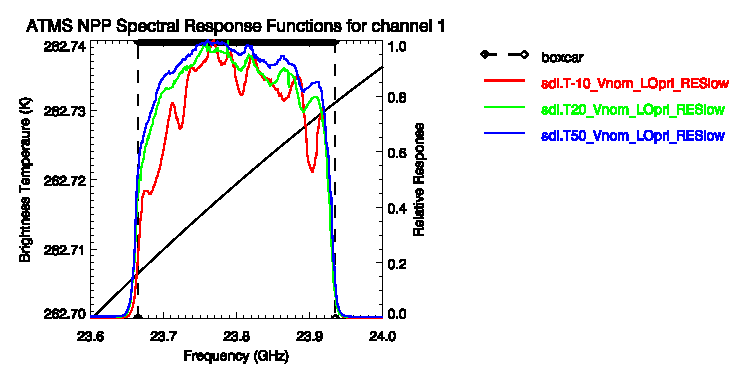
\includegraphics[bb=80 400 280 558,clip,scale=0.85]{graphics/srf/Tset/atms_npp.ch1.osrf.eps} &
    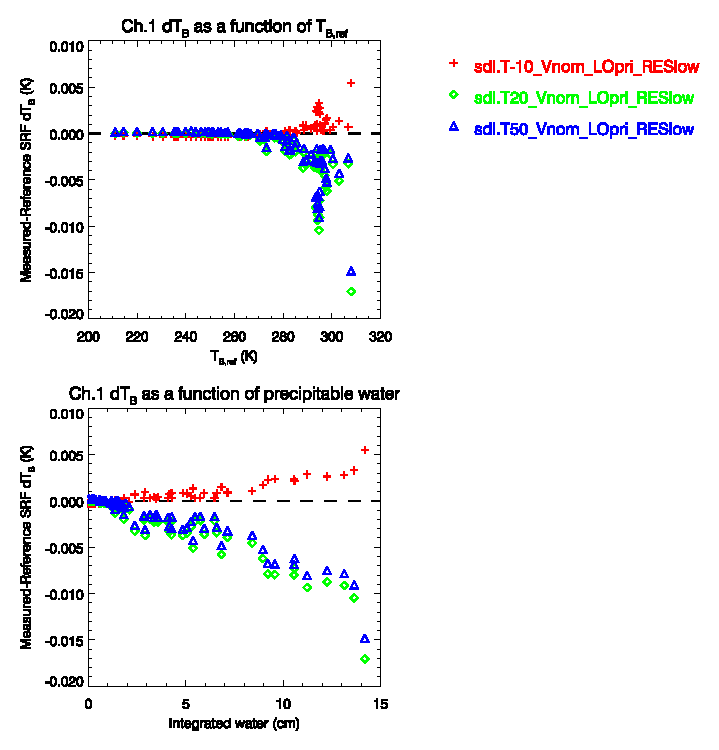
\includegraphics[bb=85 400 260 558,clip,scale=0.85]{graphics/dtb/Tset/e1.0_r0.0/atms_npp.ch1.dTb.eps} & 
    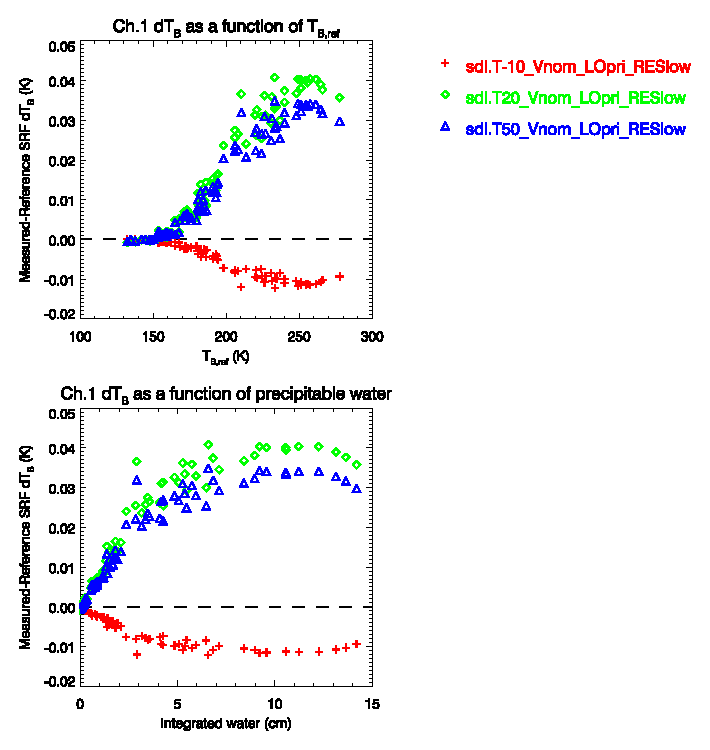
\includegraphics[bb=85 400 290 558,clip,scale=0.85]{graphics/dtb/Tset/e0.6_r0.4/atms_npp.ch1.dTb.eps} 
  \end{tabular} \\
  % the hand-crafted legend
  \setlength{\unitlength}{1cm}
  \begin{picture}(8.0,1.0)
    \thicklines
    \color{red}
    \put(0.0,0.5){\line(1,0){1}}
    \put(1.2,0.35){\sffamily \textbf{+}\quad -10\textdegree{}C}
    \color{green}
    \put(3.0,0.5){\line(1,0){1}}
    \put(4.2,0.35){\sffamily {\Large$\diamond$}\quad 20\textdegree{}C}
    \color{blue}
    \put(6.0,0.5){\line(1,0){1}}
    \put(7.2,0.35){\sffamily $\bigtriangleup$\quad 50\textdegree{}C}
  \end{picture}
  \caption{Channel 1 NPP ATMS \textbf{(a)} SRF data digitized from plots in the ATMS PFM Calibration Data Book\cite{ATMS_PFM_CalLog} with the corresponding boxcar response based on table \ref{tab:atms_fo_sb_and_df}. A representative brightness temperature spectrum is also shown. \textbf{(b)} Difference in the MonoRTM-derived brightness temperatures, using unity surface emissivity, as a function of the boxcar SRF $T_B$ for nominal bias voltage and three baseplate temperatures (-10, 20, and 50\textdegree{}C). \textbf{(c)} Same as (b), but for surface emissivity and reflectivity of 0.6 and 0.4 respectively. }
  \label{fig:atms_npp.Tset.ch1}
\end{figure}

\begin{figure}[H]
  \centering
  \begin{tabular}{c c c}
    \textsf{\textbf{(a)} SRFs} &
    \textsf{\textbf{(b)} $\Delta T_B$ $(\epsilon_s = 1.0)$} &
    \textsf{\textbf{(c)} $\Delta T_B$ $(\epsilon_s = 0.6)$} \\
    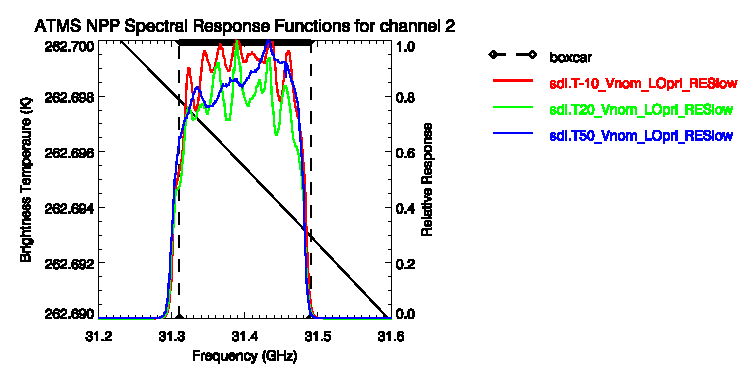
\includegraphics[bb=80 400 280 558,clip,scale=0.85]{graphics/srf/Tset/atms_npp.ch2.osrf.eps} &
    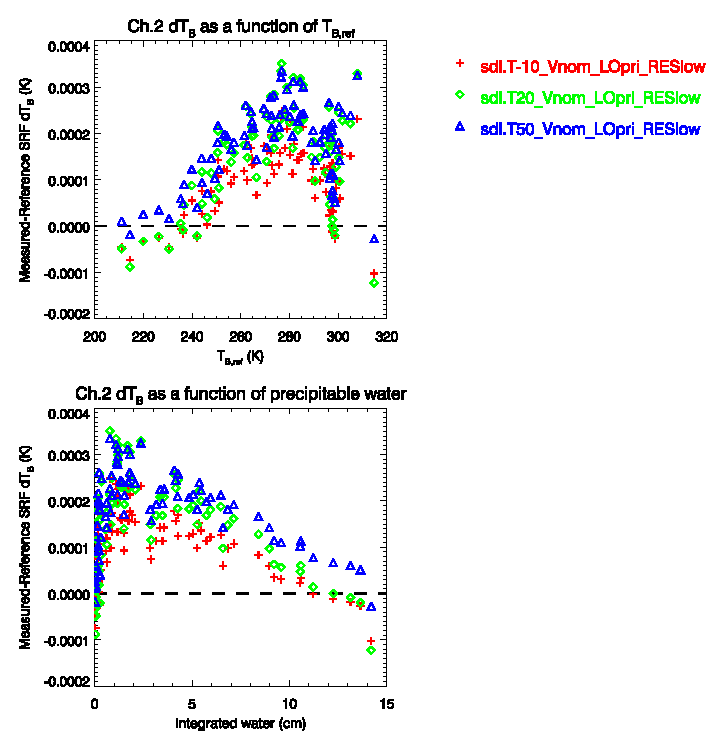
\includegraphics[bb=85 400 260 558,clip,scale=0.85]{graphics/dtb/Tset/e1.0_r0.0/atms_npp.ch2.dTb.eps} & 
    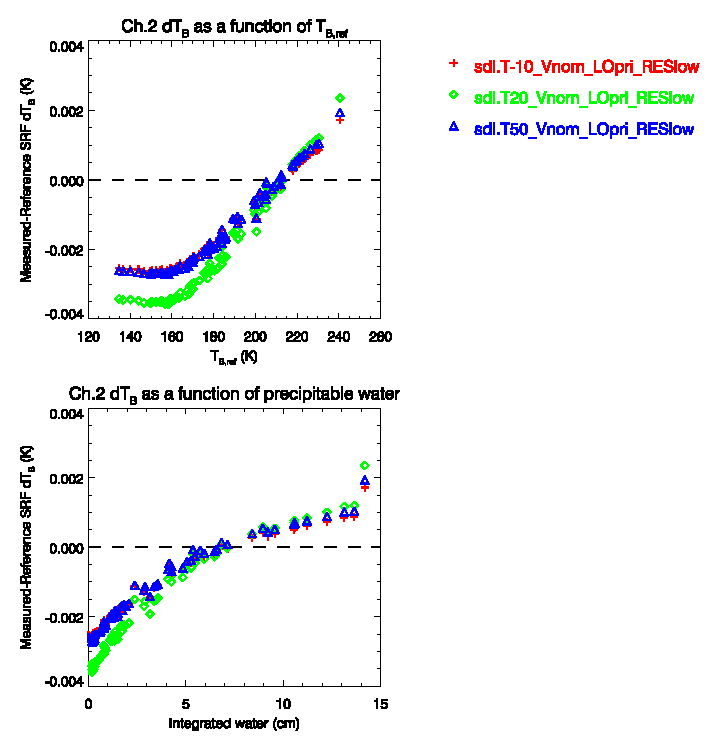
\includegraphics[bb=85 400 290 558,clip,scale=0.85]{graphics/dtb/Tset/e0.6_r0.4/atms_npp.ch2.dTb.eps} 
  \end{tabular} \\
  % the hand-crafted legend
  \setlength{\unitlength}{1cm}
  \begin{picture}(8.0,1.0)
    \thicklines
    \color{red}
    \put(0.0,0.5){\line(1,0){1}}
    \put(1.2,0.35){\sffamily \textbf{+}\quad -10\textdegree{}C}
    \color{green}
    \put(3.0,0.5){\line(1,0){1}}
    \put(4.2,0.35){\sffamily {\Large$\diamond$}\quad 20\textdegree{}C}
    \color{blue}
    \put(6.0,0.5){\line(1,0){1}}
    \put(7.2,0.35){\sffamily $\bigtriangleup$\quad 50\textdegree{}C}
  \end{picture}
  \caption{Channel 2 NPP ATMS \textbf{(a)} SRF data digitized from plots in the ATMS PFM Calibration Data Book\cite{ATMS_PFM_CalLog} with the corresponding boxcar response based on table \ref{tab:atms_fo_sb_and_df}. A representative brightness temperature spectrum is also shown. \textbf{(b)} Difference in the MonoRTM-derived brightness temperatures, using unity surface emissivity, as a function of the boxcar SRF $T_B$ for nominal bias voltage and three baseplate temperatures (-10, 20, and 50\textdegree{}C). \textbf{(c)} Same as (b), but for surface emissivity and reflectivity of 0.6 and 0.4 respectively. }
  \label{fig:atms_npp.Tset.ch2}
\end{figure}

\begin{figure}[H]
  \centering
  \begin{tabular}{c c c}
    \textsf{\textbf{(a)} SRFs} &
    \textsf{\textbf{(b)} $\Delta T_B$ $(\epsilon_s = 1.0)$} &
    \textsf{\textbf{(c)} $\Delta T_B$ $(\epsilon_s = 0.6)$} \\
    \includegraphics[bb=80 400 280 558,clip,scale=0.85]{graphics/srf/Tset/atms_npp.ch3.osrf.eps} &
    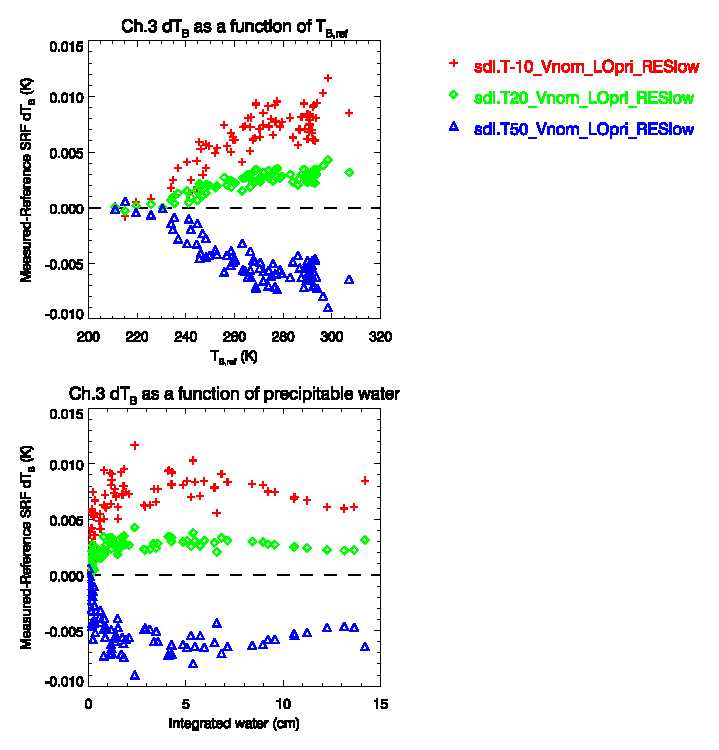
\includegraphics[bb=85 400 260 558,clip,scale=0.85]{graphics/dtb/Tset/e1.0_r0.0/atms_npp.ch3.dTb.eps} & 
    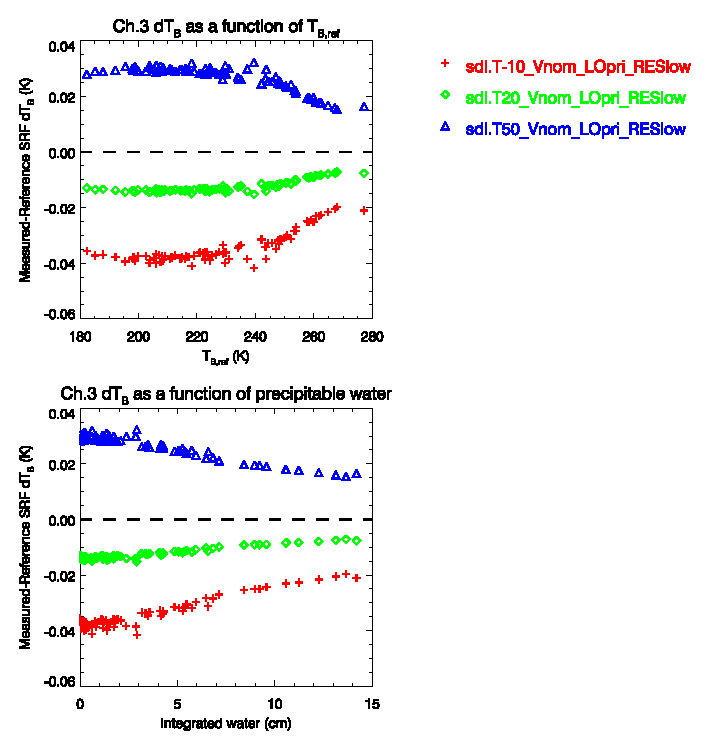
\includegraphics[bb=85 400 290 558,clip,scale=0.85]{graphics/dtb/Tset/e0.6_r0.4/atms_npp.ch3.dTb.eps} 
  \end{tabular} \\
  % the hand-crafted legend
  \setlength{\unitlength}{1cm}
  \begin{picture}(8.0,1.0)
    \thicklines
    \color{red}
    \put(0.0,0.5){\line(1,0){1}}
    \put(1.2,0.35){\sffamily \textbf{+}\quad -10\textdegree{}C}
    \color{green}
    \put(3.0,0.5){\line(1,0){1}}
    \put(4.2,0.35){\sffamily {\Large$\diamond$}\quad 20\textdegree{}C}
    \color{blue}
    \put(6.0,0.5){\line(1,0){1}}
    \put(7.2,0.35){\sffamily $\bigtriangleup$\quad 50\textdegree{}C}
  \end{picture}
  \caption{Channel 3 NPP ATMS \textbf{(a)} SRF data digitized from plots in the ATMS PFM Calibration Data Book\cite{ATMS_PFM_CalLog} with the corresponding boxcar response based on table \ref{tab:atms_fo_sb_and_df}. A representative brightness temperature spectrum is also shown. \textbf{(b)} Difference in the MonoRTM-derived brightness temperatures, using unity surface emissivity, as a function of the boxcar SRF $T_B$ for nominal bias voltage and three baseplate temperatures (-10, 20, and 50\textdegree{}C). \textbf{(c)} Same as (b), but for surface emissivity and reflectivity of 0.6 and 0.4 respectively. }
  \label{fig:atms_npp.Tset.ch3}
\end{figure}

\begin{figure}[H]
  \centering
  \begin{tabular}{c c c}
    \textsf{\textbf{(a)} SRFs} &
    \textsf{\textbf{(b)} $\Delta T_B$ $(\epsilon_s = 1.0)$} &
    \textsf{\textbf{(c)} $\Delta T_B$ $(\epsilon_s = 0.6)$} \\
    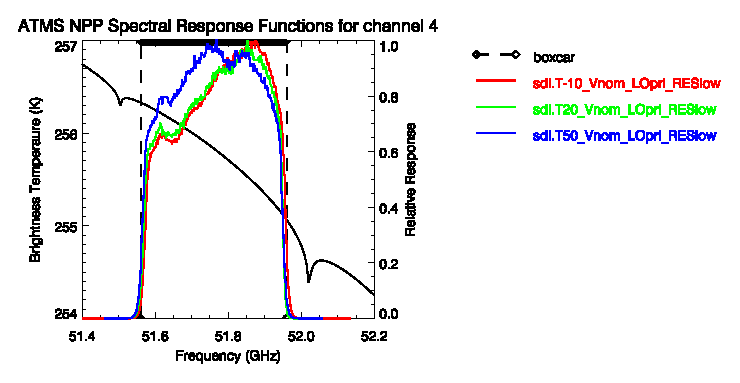
\includegraphics[bb=80 400 280 558,clip,scale=0.85]{graphics/srf/Tset/atms_npp.ch4.osrf.eps} &
    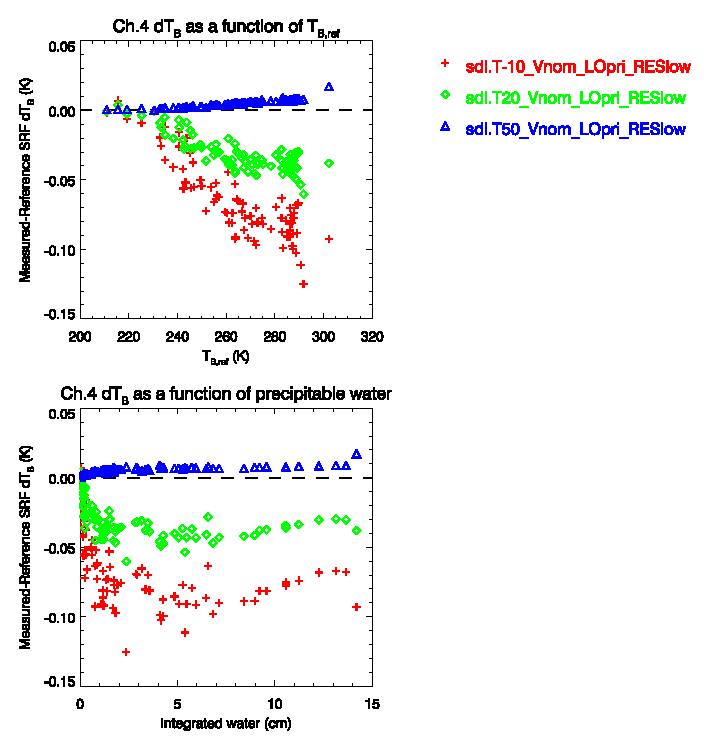
\includegraphics[bb=85 400 260 558,clip,scale=0.85]{graphics/dtb/Tset/e1.0_r0.0/atms_npp.ch4.dTb.eps} & 
    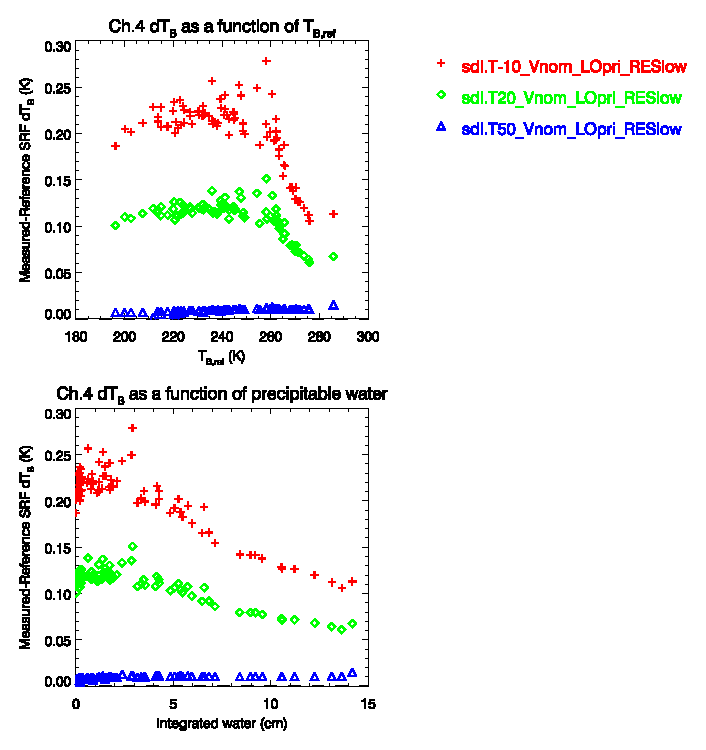
\includegraphics[bb=85 400 290 558,clip,scale=0.85]{graphics/dtb/Tset/e0.6_r0.4/atms_npp.ch4.dTb.eps} 
  \end{tabular} \\
  % the hand-crafted legend
  \setlength{\unitlength}{1cm}
  \begin{picture}(8.0,1.0)
    \thicklines
    \color{red}
    \put(0.0,0.5){\line(1,0){1}}
    \put(1.2,0.35){\sffamily \textbf{+}\quad -10\textdegree{}C}
    \color{green}
    \put(3.0,0.5){\line(1,0){1}}
    \put(4.2,0.35){\sffamily {\Large$\diamond$}\quad 20\textdegree{}C}
    \color{blue}
    \put(6.0,0.5){\line(1,0){1}}
    \put(7.2,0.35){\sffamily $\bigtriangleup$\quad 50\textdegree{}C}
  \end{picture}
  \caption{Channel 4 NPP ATMS \textbf{(a)} SRF data digitized from plots in the ATMS PFM Calibration Data Book\cite{ATMS_PFM_CalLog} with the corresponding boxcar response based on table \ref{tab:atms_fo_sb_and_df}. A representative brightness temperature spectrum is also shown. \textbf{(b)} Difference in the MonoRTM-derived brightness temperatures, using unity surface emissivity, as a function of the boxcar SRF $T_B$ for nominal bias voltage and three baseplate temperatures (-10, 20, and 50\textdegree{}C). \textbf{(c)} Same as (b), but for surface emissivity and reflectivity of 0.6 and 0.4 respectively. }
  \label{fig:atms_npp.Tset.ch4}
\end{figure}

\begin{figure}[H]
  \centering
  \begin{tabular}{c c c}
    \textsf{\textbf{(a)} SRFs} &
    \textsf{\textbf{(b)} $\Delta T_B$ $(\epsilon_s = 1.0)$} &
    \textsf{\textbf{(c)} $\Delta T_B$ $(\epsilon_s = 0.6)$} \\
    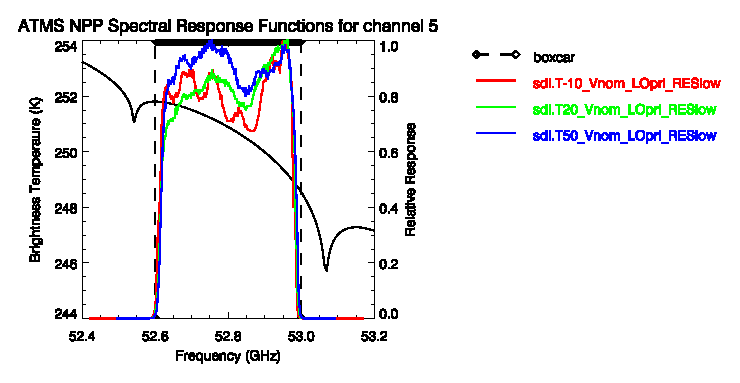
\includegraphics[bb=80 400 280 558,clip,scale=0.85]{graphics/srf/Tset/atms_npp.ch5.osrf.eps} &
    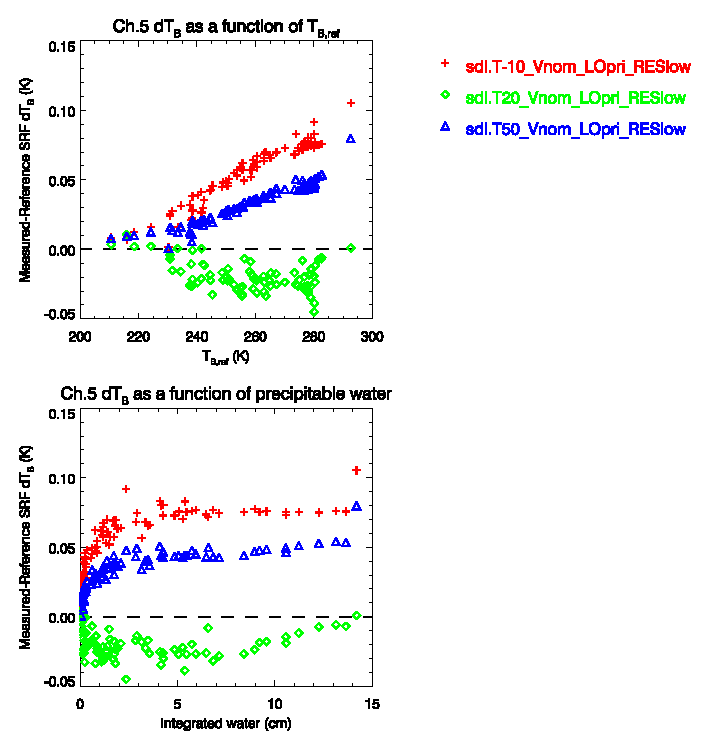
\includegraphics[bb=85 400 260 558,clip,scale=0.85]{graphics/dtb/Tset/e1.0_r0.0/atms_npp.ch5.dTb.eps} & 
    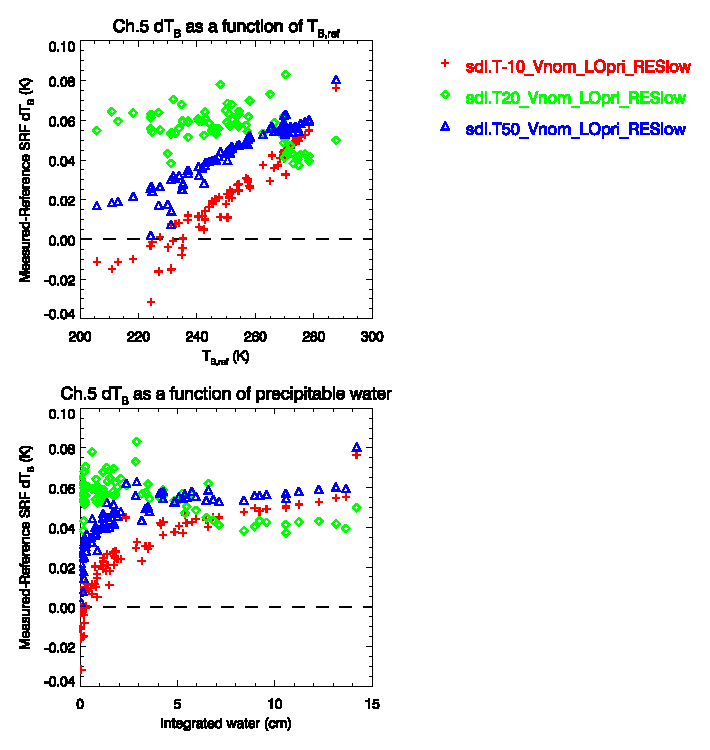
\includegraphics[bb=85 400 290 558,clip,scale=0.85]{graphics/dtb/Tset/e0.6_r0.4/atms_npp.ch5.dTb.eps} 
  \end{tabular} \\
  % the hand-crafted legend
  \setlength{\unitlength}{1cm}
  \begin{picture}(8.0,1.0)
    \thicklines
    \color{red}
    \put(0.0,0.5){\line(1,0){1}}
    \put(1.2,0.35){\sffamily \textbf{+}\quad -10\textdegree{}C}
    \color{green}
    \put(3.0,0.5){\line(1,0){1}}
    \put(4.2,0.35){\sffamily {\Large$\diamond$}\quad 20\textdegree{}C}
    \color{blue}
    \put(6.0,0.5){\line(1,0){1}}
    \put(7.2,0.35){\sffamily $\bigtriangleup$\quad 50\textdegree{}C}
  \end{picture}
  \caption{Channel 5 NPP ATMS \textbf{(a)} SRF data digitized from plots in the ATMS PFM Calibration Data Book\cite{ATMS_PFM_CalLog} with the corresponding boxcar response based on table \ref{tab:atms_fo_sb_and_df}. A representative brightness temperature spectrum is also shown. \textbf{(b)} Difference in the MonoRTM-derived brightness temperatures, using unity surface emissivity, as a function of the boxcar SRF $T_B$ for nominal bias voltage and three baseplate temperatures (-10, 20, and 50\textdegree{}C). \textbf{(c)} Same as (b), but for surface emissivity and reflectivity of 0.6 and 0.4 respectively. }
  \label{fig:atms_npp.Tset.ch5}
\end{figure}

\begin{figure}[H]
  \centering
  \begin{tabular}{c c c}
    \textsf{\textbf{(a)} SRFs} &
    \textsf{\textbf{(b)} $\Delta T_B$ $(\epsilon_s = 1.0)$} &
    \textsf{\textbf{(c)} $\Delta T_B$ $(\epsilon_s = 0.6)$} \\
    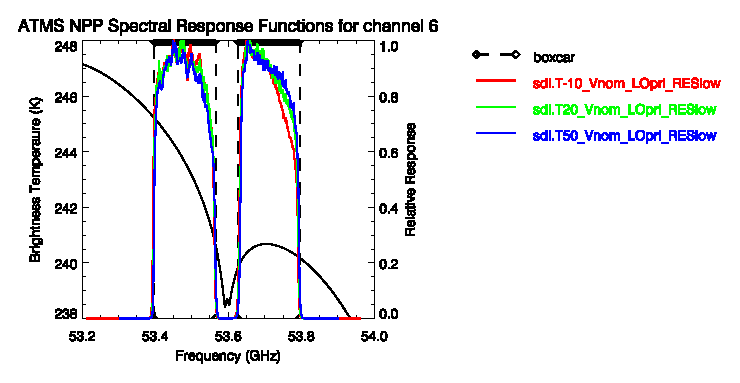
\includegraphics[bb=80 400 280 558,clip,scale=0.85]{graphics/srf/Tset/atms_npp.ch6.osrf.eps} &
    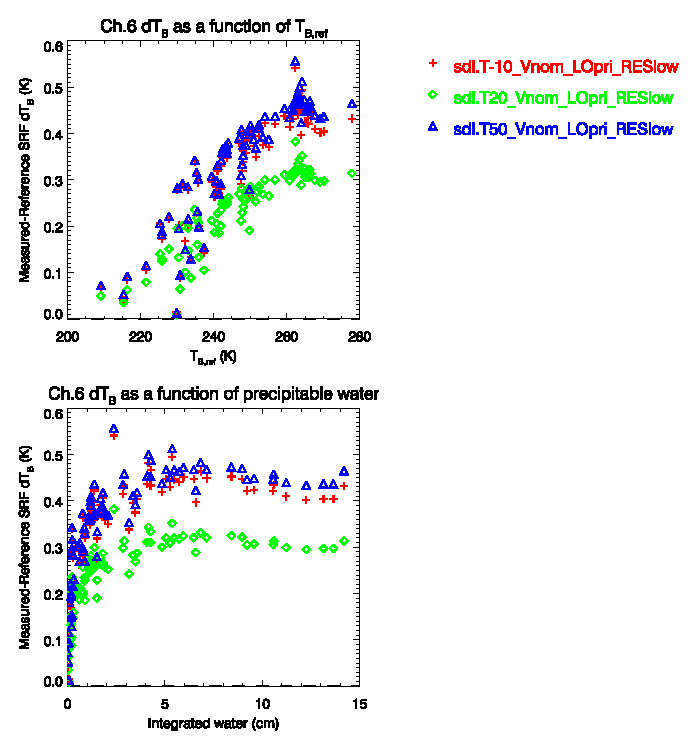
\includegraphics[bb=85 400 260 558,clip,scale=0.85]{graphics/dtb/Tset/e1.0_r0.0/atms_npp.ch6.dTb.eps} & 
    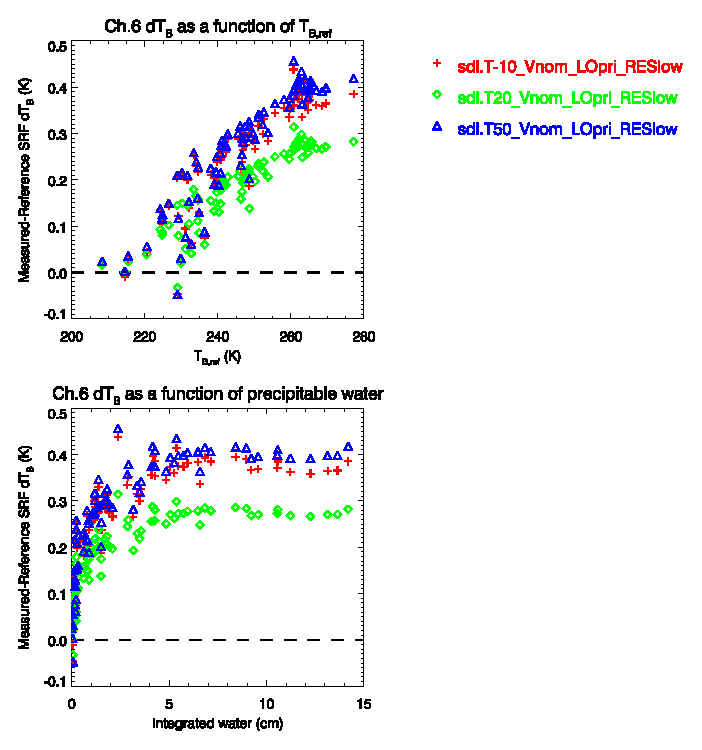
\includegraphics[bb=85 400 290 558,clip,scale=0.85]{graphics/dtb/Tset/e0.6_r0.4/atms_npp.ch6.dTb.eps} 
  \end{tabular} \\
  % the hand-crafted legend
  \setlength{\unitlength}{1cm}
  \begin{picture}(8.0,1.0)
    \thicklines
    \color{red}
    \put(0.0,0.5){\line(1,0){1}}
    \put(1.2,0.35){\sffamily \textbf{+}\quad -10\textdegree{}C}
    \color{green}
    \put(3.0,0.5){\line(1,0){1}}
    \put(4.2,0.35){\sffamily {\Large$\diamond$}\quad 20\textdegree{}C}
    \color{blue}
    \put(6.0,0.5){\line(1,0){1}}
    \put(7.2,0.35){\sffamily $\bigtriangleup$\quad 50\textdegree{}C}
  \end{picture}
  \caption{Channel 6 NPP ATMS \textbf{(a)} SRF data digitized from plots in the ATMS PFM Calibration Data Book\cite{ATMS_PFM_CalLog} with the corresponding boxcar response based on table \ref{tab:atms_fo_sb_and_df}. A representative brightness temperature spectrum is also shown. \textbf{(b)} Difference in the MonoRTM-derived brightness temperatures, using unity surface emissivity, as a function of the boxcar SRF $T_B$ for nominal bias voltage and three baseplate temperatures (-10, 20, and 50\textdegree{}C). \textbf{(c)} Same as (b), but for surface emissivity and reflectivity of 0.6 and 0.4 respectively. }
  \label{fig:atms_npp.Tset.ch6}
\end{figure}

\begin{figure}[H]
  \centering
  \begin{tabular}{c c c}
    \textsf{\textbf{(a)} SRFs} &
    \textsf{\textbf{(b)} $\Delta T_B$ $(\epsilon_s = 1.0)$} &
    \textsf{\textbf{(c)} $\Delta T_B$ $(\epsilon_s = 0.6)$} \\
    \includegraphics[bb=80 400 280 558,clip,scale=0.85]{graphics/srf/Tset/atms_npp.ch7.osrf.eps} &
    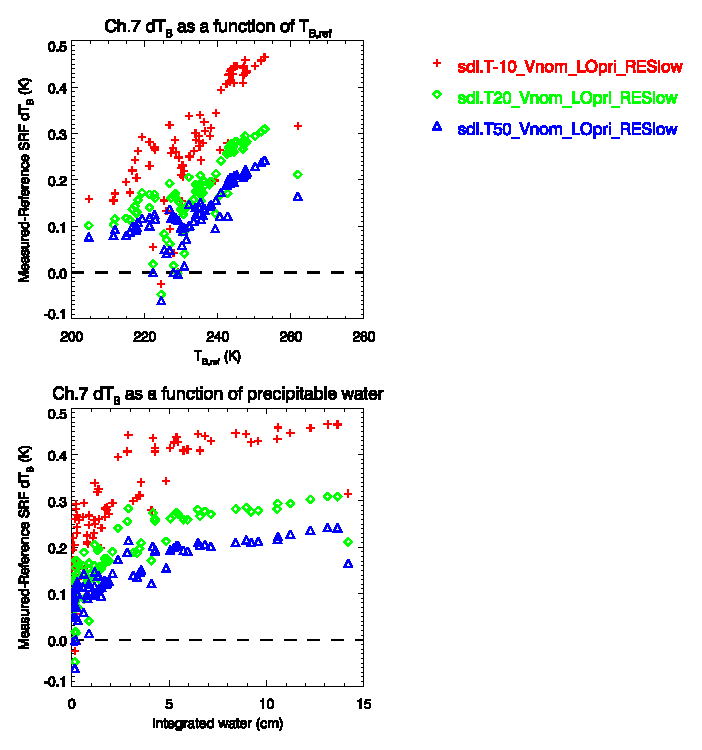
\includegraphics[bb=85 400 260 558,clip,scale=0.85]{graphics/dtb/Tset/e1.0_r0.0/atms_npp.ch7.dTb.eps} & 
    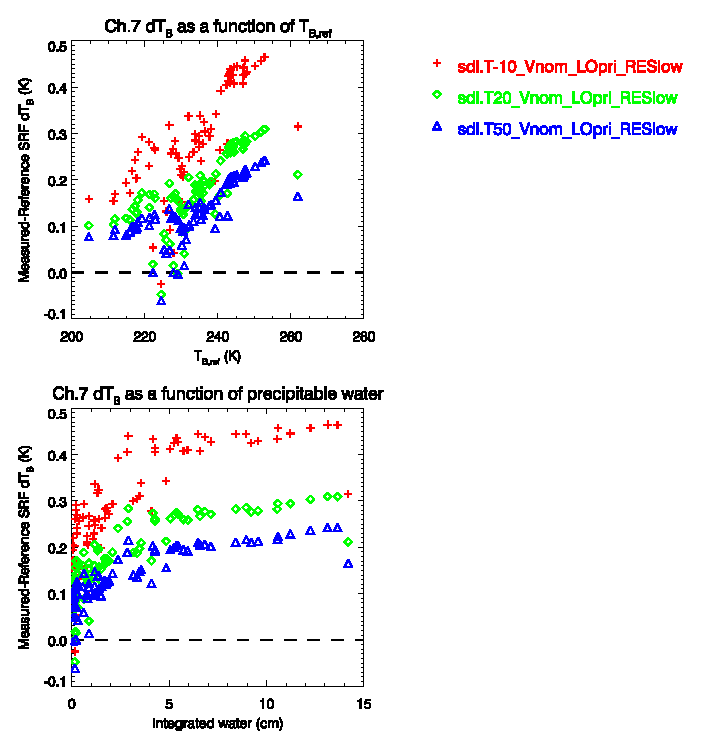
\includegraphics[bb=85 400 290 558,clip,scale=0.85]{graphics/dtb/Tset/e0.6_r0.4/atms_npp.ch7.dTb.eps} 
  \end{tabular} \\
  % the hand-crafted legend
  \setlength{\unitlength}{1cm}
  \begin{picture}(8.0,1.0)
    \thicklines
    \color{red}
    \put(0.0,0.5){\line(1,0){1}}
    \put(1.2,0.35){\sffamily \textbf{+}\quad -10\textdegree{}C}
    \color{green}
    \put(3.0,0.5){\line(1,0){1}}
    \put(4.2,0.35){\sffamily {\Large$\diamond$}\quad 20\textdegree{}C}
    \color{blue}
    \put(6.0,0.5){\line(1,0){1}}
    \put(7.2,0.35){\sffamily $\bigtriangleup$\quad 50\textdegree{}C}
  \end{picture}
  \caption{Channel 7 NPP ATMS \textbf{(a)} SRF data digitized from plots in the ATMS PFM Calibration Data Book\cite{ATMS_PFM_CalLog} with the corresponding boxcar response based on table \ref{tab:atms_fo_sb_and_df}. A representative brightness temperature spectrum is also shown. \textbf{(b)} Difference in the MonoRTM-derived brightness temperatures, using unity surface emissivity, as a function of the boxcar SRF $T_B$ for nominal bias voltage and three baseplate temperatures (-10, 20, and 50\textdegree{}C). \textbf{(c)} Same as (b), but for surface emissivity and reflectivity of 0.6 and 0.4 respectively. }
  \label{fig:atms_npp.Tset.ch7}
\end{figure}

\begin{figure}[H]
  \centering
  \begin{tabular}{c c c}
    \textsf{\textbf{(a)} SRFs} &
    \textsf{\textbf{(b)} $\Delta T_B$ $(\epsilon_s = 1.0)$} &
    \textsf{\textbf{(c)} $\Delta T_B$ $(\epsilon_s = 0.6)$} \\
    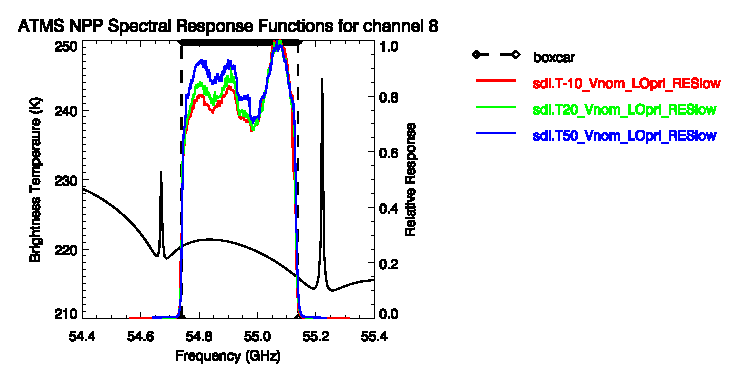
\includegraphics[bb=80 400 280 558,clip,scale=0.85]{graphics/srf/Tset/atms_npp.ch8.osrf.eps} &
    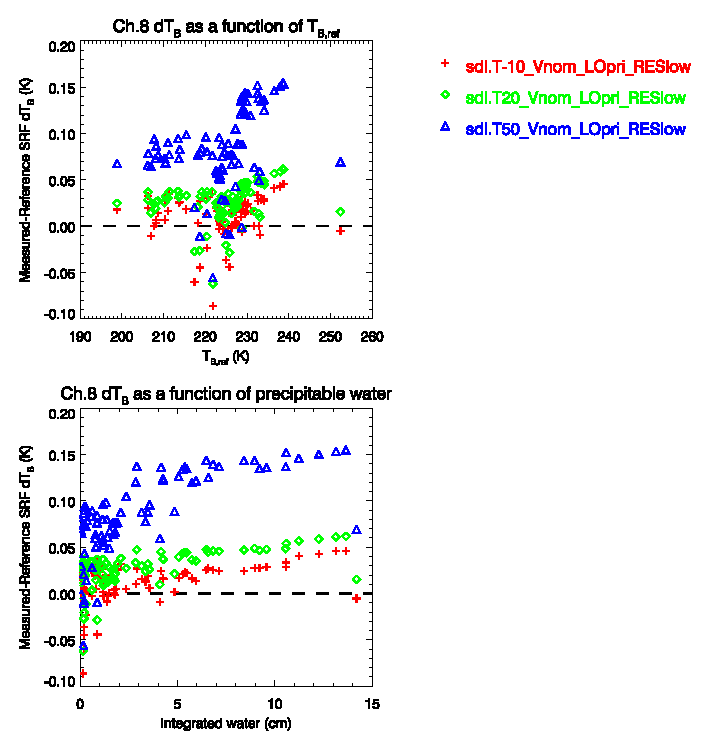
\includegraphics[bb=85 400 260 558,clip,scale=0.85]{graphics/dtb/Tset/e1.0_r0.0/atms_npp.ch8.dTb.eps} & 
    \includegraphics[bb=85 400 290 558,clip,scale=0.85]{graphics/dtb/Tset/e0.6_r0.4/atms_npp.ch8.dTb.eps} 
  \end{tabular} \\
  % the hand-crafted legend
  \setlength{\unitlength}{1cm}
  \begin{picture}(8.0,1.0)
    \thicklines
    \color{red}
    \put(0.0,0.5){\line(1,0){1}}
    \put(1.2,0.35){\sffamily \textbf{+}\quad -10\textdegree{}C}
    \color{green}
    \put(3.0,0.5){\line(1,0){1}}
    \put(4.2,0.35){\sffamily {\Large$\diamond$}\quad 20\textdegree{}C}
    \color{blue}
    \put(6.0,0.5){\line(1,0){1}}
    \put(7.2,0.35){\sffamily $\bigtriangleup$\quad 50\textdegree{}C}
  \end{picture}
  \caption{Channel 8 NPP ATMS \textbf{(a)} SRF data digitized from plots in the ATMS PFM Calibration Data Book\cite{ATMS_PFM_CalLog} with the corresponding boxcar response based on table \ref{tab:atms_fo_sb_and_df}. A representative brightness temperature spectrum is also shown. \textbf{(b)} Difference in the MonoRTM-derived brightness temperatures, using unity surface emissivity, as a function of the boxcar SRF $T_B$ for nominal bias voltage and three baseplate temperatures (-10, 20, and 50\textdegree{}C). \textbf{(c)} Same as (b), but for surface emissivity and reflectivity of 0.6 and 0.4 respectively. }
  \label{fig:atms_npp.Tset.ch8}
\end{figure}

\begin{figure}[H]
  \centering
  \begin{tabular}{c c c}
    \textsf{\textbf{(a)} SRFs} &
    \textsf{\textbf{(b)} $\Delta T_B$ $(\epsilon_s = 1.0)$} &
    \textsf{\textbf{(c)} $\Delta T_B$ $(\epsilon_s = 0.6)$} \\
    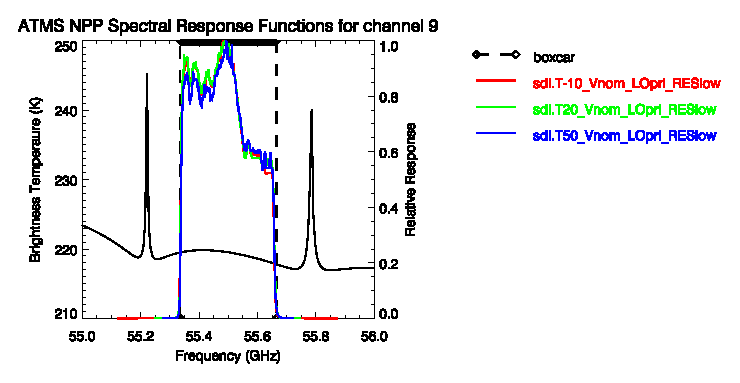
\includegraphics[bb=80 400 280 558,clip,scale=0.85]{graphics/srf/Tset/atms_npp.ch9.osrf.eps} &
    \includegraphics[bb=85 400 260 558,clip,scale=0.85]{graphics/dtb/Tset/e1.0_r0.0/atms_npp.ch9.dTb.eps} & 
    \includegraphics[bb=85 400 290 558,clip,scale=0.85]{graphics/dtb/Tset/e0.6_r0.4/atms_npp.ch9.dTb.eps} 
  \end{tabular} \\
  % the hand-crafted legend
  \setlength{\unitlength}{1cm}
  \begin{picture}(8.0,1.0)
    \thicklines
    \color{red}
    \put(0.0,0.5){\line(1,0){1}}
    \put(1.2,0.35){\sffamily \textbf{+}\quad -10\textdegree{}C}
    \color{green}
    \put(3.0,0.5){\line(1,0){1}}
    \put(4.2,0.35){\sffamily {\Large$\diamond$}\quad 20\textdegree{}C}
    \color{blue}
    \put(6.0,0.5){\line(1,0){1}}
    \put(7.2,0.35){\sffamily $\bigtriangleup$\quad 50\textdegree{}C}
  \end{picture}
  \caption{Channel 9 NPP ATMS \textbf{(a)} SRF data digitized from plots in the ATMS PFM Calibration Data Book\cite{ATMS_PFM_CalLog} with the corresponding boxcar response based on table \ref{tab:atms_fo_sb_and_df}. A representative brightness temperature spectrum is also shown. \textbf{(b)} Difference in the MonoRTM-derived brightness temperatures, using unity surface emissivity, as a function of the boxcar SRF $T_B$ for nominal bias voltage and three baseplate temperatures (-10, 20, and 50\textdegree{}C). \textbf{(c)} Same as (b), but for surface emissivity and reflectivity of 0.6 and 0.4 respectively. }
  \label{fig:atms_npp.Tset.ch9}
\end{figure}

\begin{figure}[H]
  \centering
  \begin{tabular}{c c c}
    \textsf{\textbf{(a)} SRFs} &
    \textsf{\textbf{(b)} $\Delta T_B$ $(\epsilon_s = 1.0)$} &
    \textsf{\textbf{(c)} $\Delta T_B$ $(\epsilon_s = 0.6)$} \\
    \includegraphics[bb=80 400 280 558,clip,scale=0.85]{graphics/srf/Tset/atms_npp.ch10.osrf.eps} &
    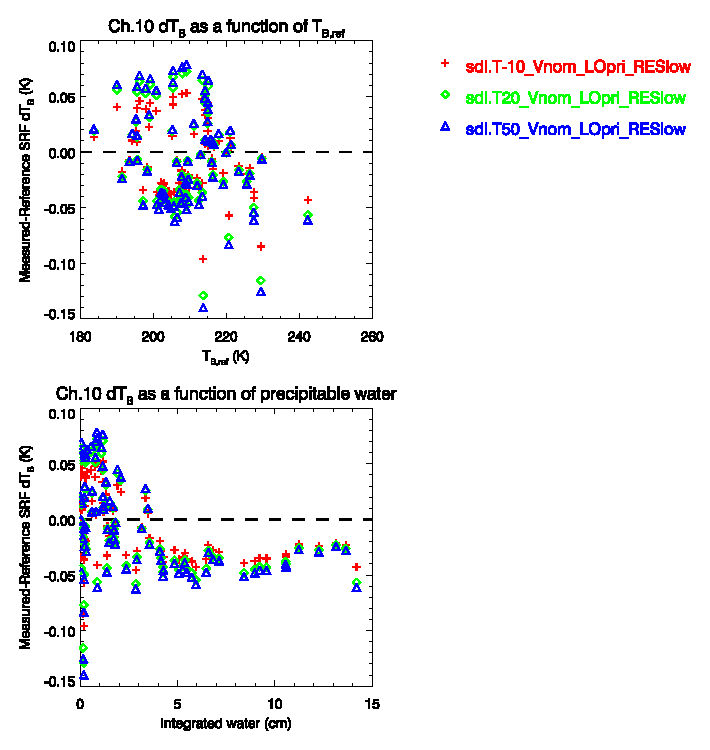
\includegraphics[bb=85 400 260 558,clip,scale=0.85]{graphics/dtb/Tset/e1.0_r0.0/atms_npp.ch10.dTb.eps} & 
    \includegraphics[bb=85 400 290 558,clip,scale=0.85]{graphics/dtb/Tset/e0.6_r0.4/atms_npp.ch10.dTb.eps} 
  \end{tabular} \\
  % the hand-crafted legend
  \setlength{\unitlength}{1cm}
  \begin{picture}(8.0,1.0)
    \thicklines
    \color{red}
    \put(0.0,0.5){\line(1,0){1}}
    \put(1.2,0.35){\sffamily \textbf{+}\quad -10\textdegree{}C}
    \color{green}
    \put(3.0,0.5){\line(1,0){1}}
    \put(4.2,0.35){\sffamily {\Large$\diamond$}\quad 20\textdegree{}C}
    \color{blue}
    \put(6.0,0.5){\line(1,0){1}}
    \put(7.2,0.35){\sffamily $\bigtriangleup$\quad 50\textdegree{}C}
  \end{picture}
  \caption{Channel 10 NPP ATMS \textbf{(a)} SRF data digitized from plots in the ATMS PFM Calibration Data Book\cite{ATMS_PFM_CalLog} with the corresponding boxcar response based on table \ref{tab:atms_fo_sb_and_df}. A representative brightness temperature spectrum is also shown. \textbf{(b)} Difference in the MonoRTM-derived brightness temperatures, using unity surface emissivity, as a function of the boxcar SRF $T_B$ for nominal bias voltage and three baseplate temperatures (-10, 20, and 50\textdegree{}C). \textbf{(c)} Same as (b), but for surface emissivity and reflectivity of 0.6 and 0.4 respectively. }
  \label{fig:atms_npp.Tset.ch10}
\end{figure}

\begin{figure}[H]
  \centering
  \begin{tabular}{c c c}
    \textsf{\textbf{(a)} SRFs} &
    \textsf{\textbf{(b)} $\Delta T_B$ $(\epsilon_s = 1.0)$} &
    \textsf{\textbf{(c)} $\Delta T_B$ $(\epsilon_s = 0.6)$} \\
    \includegraphics[bb=80 400 280 558,clip,scale=0.85]{graphics/srf/Tset/atms_npp.ch11.osrf.eps} &
    \includegraphics[bb=85 400 260 558,clip,scale=0.85]{graphics/dtb/Tset/e1.0_r0.0/atms_npp.ch11.dTb.eps} & 
    \includegraphics[bb=85 400 290 558,clip,scale=0.85]{graphics/dtb/Tset/e0.6_r0.4/atms_npp.ch11.dTb.eps} 
  \end{tabular} \\
  % the hand-crafted legend
  \setlength{\unitlength}{1cm}
  \begin{picture}(8.0,1.0)
    \thicklines
    \color{red}
    \put(0.0,0.5){\line(1,0){1}}
    \put(1.2,0.35){\sffamily \textbf{+}\quad -10\textdegree{}C}
    \color{green}
    \put(3.0,0.5){\line(1,0){1}}
    \put(4.2,0.35){\sffamily {\Large$\diamond$}\quad 20\textdegree{}C}
    \color{blue}
    \put(6.0,0.5){\line(1,0){1}}
    \put(7.2,0.35){\sffamily $\bigtriangleup$\quad 50\textdegree{}C}
  \end{picture}
  \caption{Channel 11 NPP ATMS \textbf{(a)} SRF data digitized from plots in the ATMS PFM Calibration Data Book\cite{ATMS_PFM_CalLog} with the corresponding boxcar response based on table \ref{tab:atms_fo_sb_and_df}. A representative brightness temperature spectrum is also shown. \textbf{(b)} Difference in the MonoRTM-derived brightness temperatures, using unity surface emissivity, as a function of the boxcar SRF $T_B$ for nominal bias voltage and three baseplate temperatures (-10, 20, and 50\textdegree{}C). \textbf{(c)} Same as (b), but for surface emissivity and reflectivity of 0.6 and 0.4 respectively. }
  \label{fig:atms_npp.Tset.ch11}
\end{figure}

\begin{figure}[H]
  \centering
  \begin{tabular}{c c c}
    \textsf{\textbf{(a)} SRFs (low $f$ passbands only)} &
    \textsf{\textbf{(b)} $\Delta T_B$ $(\epsilon_s = 1.0)$} &
    \textsf{\textbf{(c)} $\Delta T_B$ $(\epsilon_s = 0.6)$} \\
    \includegraphics[bb=80 400 280 558,clip,scale=0.85]{graphics/srf/Tset/atms_npp.ch12.osrf.eps} &
    \includegraphics[bb=85 400 260 558,clip,scale=0.85]{graphics/dtb/Tset/e1.0_r0.0/atms_npp.ch12.dTb.eps} & 
    \includegraphics[bb=85 400 290 558,clip,scale=0.85]{graphics/dtb/Tset/e0.6_r0.4/atms_npp.ch12.dTb.eps} 
  \end{tabular} \\
  % the hand-crafted legend
  \setlength{\unitlength}{1cm}
  \begin{picture}(8.0,1.0)
    \thicklines
    \color{red}
    \put(0.0,0.5){\line(1,0){1}}
    \put(1.2,0.35){\sffamily \textbf{+}\quad -10\textdegree{}C}
    \color{green}
    \put(3.0,0.5){\line(1,0){1}}
    \put(4.2,0.35){\sffamily {\Large$\diamond$}\quad 20\textdegree{}C}
    \color{blue}
    \put(6.0,0.5){\line(1,0){1}}
    \put(7.2,0.35){\sffamily $\bigtriangleup$\quad 50\textdegree{}C}
  \end{picture}
  \caption{Channel 12 NPP ATMS \textbf{(a)} SRF data digitized from plots in the ATMS PFM Calibration Data Book\cite{ATMS_PFM_CalLog} with the corresponding boxcar response based on table \ref{tab:atms_fo_sb_and_df}. A representative brightness temperature spectrum is also shown. \textbf{(b)} Difference in the MonoRTM-derived brightness temperatures, using unity surface emissivity, as a function of the boxcar SRF $T_B$ for nominal bias voltage and three baseplate temperatures (-10, 20, and 50\textdegree{}C). \textbf{(c)} Same as (b), but for surface emissivity and reflectivity of 0.6 and 0.4 respectively. }
  \label{fig:atms_npp.Tset.ch12}
\end{figure}

\begin{figure}[H]
  \centering
  \begin{tabular}{c c c}
    \textsf{\textbf{(a)} SRFs (low $f$ passbands only)} &
    \textsf{\textbf{(b)} $\Delta T_B$ $(\epsilon_s = 1.0)$} &
    \textsf{\textbf{(c)} $\Delta T_B$ $(\epsilon_s = 0.6)$} \\
    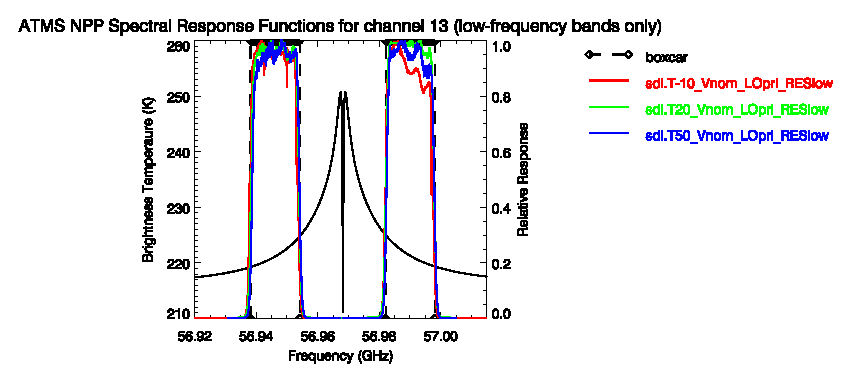
\includegraphics[bb=80 400 280 558,clip,scale=0.85]{graphics/srf/Tset/atms_npp.ch13.osrf.eps} &
    \includegraphics[bb=85 400 260 558,clip,scale=0.85]{graphics/dtb/Tset/e1.0_r0.0/atms_npp.ch13.dTb.eps} & 
    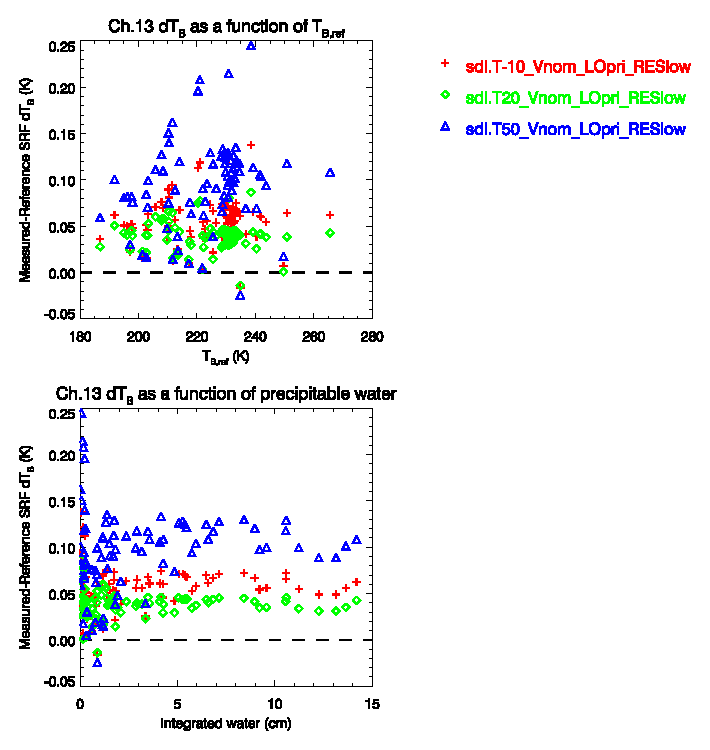
\includegraphics[bb=85 400 290 558,clip,scale=0.85]{graphics/dtb/Tset/e0.6_r0.4/atms_npp.ch13.dTb.eps} 
  \end{tabular} \\
  % the hand-crafted legend
  \setlength{\unitlength}{1cm}
  \begin{picture}(8.0,1.0)
    \thicklines
    \color{red}
    \put(0.0,0.5){\line(1,0){1}}
    \put(1.2,0.35){\sffamily \textbf{+}\quad -10\textdegree{}C}
    \color{green}
    \put(3.0,0.5){\line(1,0){1}}
    \put(4.2,0.35){\sffamily {\Large$\diamond$}\quad 20\textdegree{}C}
    \color{blue}
    \put(6.0,0.5){\line(1,0){1}}
    \put(7.2,0.35){\sffamily $\bigtriangleup$\quad 50\textdegree{}C}
  \end{picture}
  \caption{Channel 13 NPP ATMS \textbf{(a)} SRF data digitized from plots in the ATMS PFM Calibration Data Book\cite{ATMS_PFM_CalLog} with the corresponding boxcar response based on table \ref{tab:atms_fo_sb_and_df}. A representative brightness temperature spectrum is also shown. \textbf{(b)} Difference in the MonoRTM-derived brightness temperatures, using unity surface emissivity, as a function of the boxcar SRF $T_B$ for nominal bias voltage and three baseplate temperatures (-10, 20, and 50\textdegree{}C). \textbf{(c)} Same as (b), but for surface emissivity and reflectivity of 0.6 and 0.4 respectively. }
  \label{fig:atms_npp.Tset.ch13}
\end{figure}

\begin{figure}[H]
  \centering
  \begin{tabular}{c c c}
    \textsf{\textbf{(a)} SRFs (low $f$ passbands only)} &
    \textsf{\textbf{(b)} $\Delta T_B$ $(\epsilon_s = 1.0)$} &
    \textsf{\textbf{(c)} $\Delta T_B$ $(\epsilon_s = 0.6)$} \\
    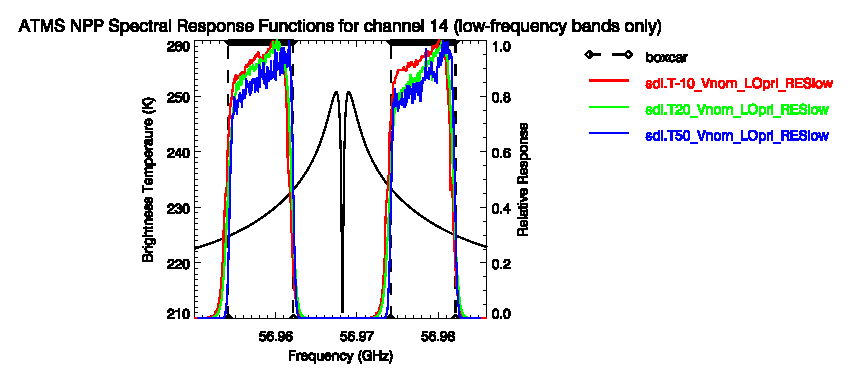
\includegraphics[bb=80 400 280 558,clip,scale=0.85]{graphics/srf/Tset/atms_npp.ch14.osrf.eps} &
    \includegraphics[bb=85 400 260 558,clip,scale=0.85]{graphics/dtb/Tset/e1.0_r0.0/atms_npp.ch14.dTb.eps} & 
    \includegraphics[bb=85 400 290 558,clip,scale=0.85]{graphics/dtb/Tset/e0.6_r0.4/atms_npp.ch14.dTb.eps} 
  \end{tabular} \\
  % the hand-crafted legend
  \setlength{\unitlength}{1cm}
  \begin{picture}(8.0,1.0)
    \thicklines
    \color{red}
    \put(0.0,0.5){\line(1,0){1}}
    \put(1.2,0.35){\sffamily \textbf{+}\quad -10\textdegree{}C}
    \color{green}
    \put(3.0,0.5){\line(1,0){1}}
    \put(4.2,0.35){\sffamily {\Large$\diamond$}\quad 20\textdegree{}C}
    \color{blue}
    \put(6.0,0.5){\line(1,0){1}}
    \put(7.2,0.35){\sffamily $\bigtriangleup$\quad 50\textdegree{}C}
  \end{picture}
  \caption{Channel 14 NPP ATMS \textbf{(a)} SRF data digitized from plots in the ATMS PFM Calibration Data Book\cite{ATMS_PFM_CalLog} with the corresponding boxcar response based on table \ref{tab:atms_fo_sb_and_df}. A representative brightness temperature spectrum is also shown. \textbf{(b)} Difference in the MonoRTM-derived brightness temperatures, using unity surface emissivity, as a function of the boxcar SRF $T_B$ for nominal bias voltage and three baseplate temperatures (-10, 20, and 50\textdegree{}C). \textbf{(c)} Same as (b), but for surface emissivity and reflectivity of 0.6 and 0.4 respectively. }
  \label{fig:atms_npp.Tset.ch14}
\end{figure}

\begin{figure}[H]
  \centering
  \begin{tabular}{c c c}
    \textsf{\textbf{(a)} SRFs (low $f$ passbands only)} &
    \textsf{\textbf{(b)} $\Delta T_B$ $(\epsilon_s = 1.0)$} &
    \textsf{\textbf{(c)} $\Delta T_B$ $(\epsilon_s = 0.6)$} \\
    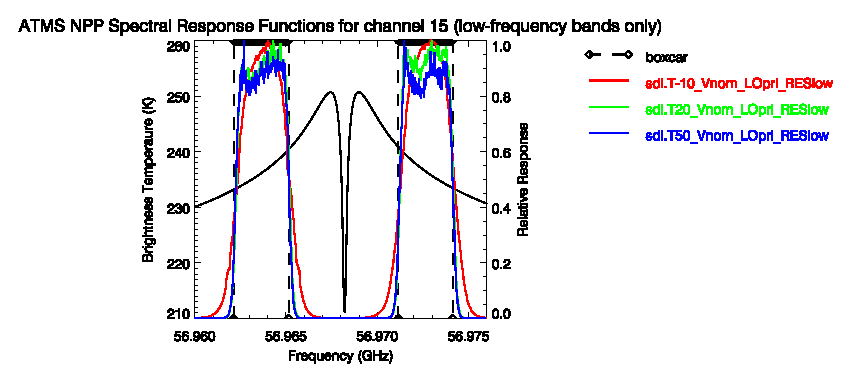
\includegraphics[bb=80 400 280 558,clip,scale=0.85]{graphics/srf/Tset/atms_npp.ch15.osrf.eps} &
    \includegraphics[bb=85 400 260 558,clip,scale=0.85]{graphics/dtb/Tset/e1.0_r0.0/atms_npp.ch15.dTb.eps} & 
    \includegraphics[bb=85 400 290 558,clip,scale=0.85]{graphics/dtb/Tset/e0.6_r0.4/atms_npp.ch15.dTb.eps} 
  \end{tabular} \\
  % the hand-crafted legend
  \setlength{\unitlength}{1cm}
  \begin{picture}(8.0,1.0)
    \thicklines
    \color{red}
    \put(0.0,0.5){\line(1,0){1}}
    \put(1.2,0.35){\sffamily \textbf{+}\quad -10\textdegree{}C}
    \color{green}
    \put(3.0,0.5){\line(1,0){1}}
    \put(4.2,0.35){\sffamily {\Large$\diamond$}\quad 20\textdegree{}C}
    \color{blue}
    \put(6.0,0.5){\line(1,0){1}}
    \put(7.2,0.35){\sffamily $\bigtriangleup$\quad 50\textdegree{}C}
  \end{picture}
  \caption{Channel 15 NPP ATMS \textbf{(a)} SRF data digitized from plots in the ATMS PFM Calibration Data Book\cite{ATMS_PFM_CalLog} with the corresponding boxcar response based on table \ref{tab:atms_fo_sb_and_df}. A representative brightness temperature spectrum is also shown. \textbf{(b)} Difference in the MonoRTM-derived brightness temperatures, using unity surface emissivity, as a function of the boxcar SRF $T_B$ for nominal bias voltage and three baseplate temperatures (-10, 20, and 50\textdegree{}C). \textbf{(c)} Same as (b), but for surface emissivity and reflectivity of 0.6 and 0.4 respectively. }
  \label{fig:atms_npp.Tset.ch15}
\end{figure}

\begin{figure}[H]
  \centering
  \begin{tabular}{c c c}
    \textsf{\textbf{(a)} SRFs} &
    \textsf{\textbf{(b)} $\Delta T_B$ $(\epsilon_s = 1.0)$} &
    \textsf{\textbf{(c)} $\Delta T_B$ $(\epsilon_s = 0.6)$} \\
    \includegraphics[bb=80 400 280 558,clip,scale=0.85]{graphics/srf/Tset/atms_npp.ch16.osrf.eps} &
    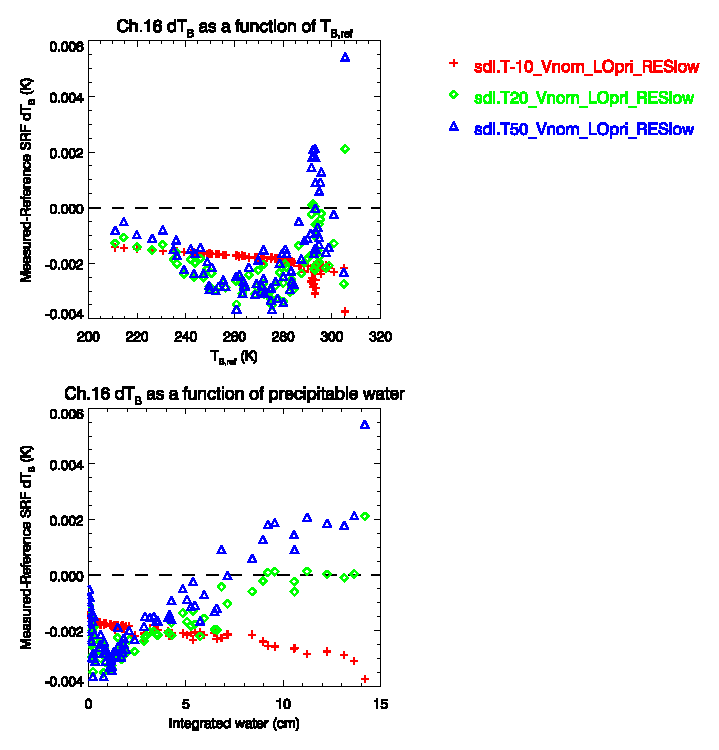
\includegraphics[bb=85 400 260 558,clip,scale=0.85]{graphics/dtb/Tset/e1.0_r0.0/atms_npp.ch16.dTb.eps} & 
    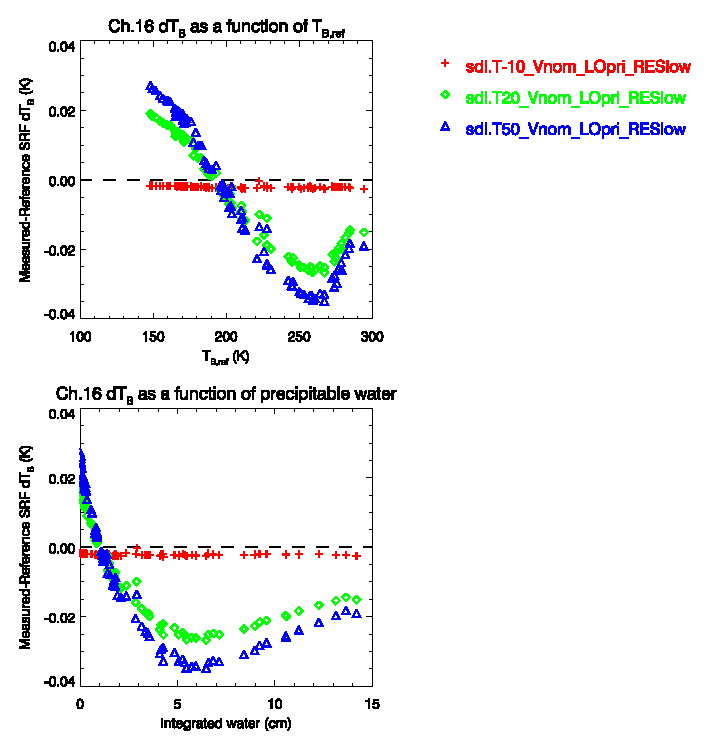
\includegraphics[bb=85 400 290 558,clip,scale=0.85]{graphics/dtb/Tset/e0.6_r0.4/atms_npp.ch16.dTb.eps} 
  \end{tabular} \\
  % the hand-crafted legend
  \setlength{\unitlength}{1cm}
  \begin{picture}(8.0,1.0)
    \thicklines
    \color{red}
    \put(0.0,0.5){\line(1,0){1}}
    \put(1.2,0.35){\sffamily \textbf{+}\quad -10\textdegree{}C}
    \color{green}
    \put(3.0,0.5){\line(1,0){1}}
    \put(4.2,0.35){\sffamily {\Large$\diamond$}\quad 20\textdegree{}C}
    \color{blue}
    \put(6.0,0.5){\line(1,0){1}}
    \put(7.2,0.35){\sffamily $\bigtriangleup$\quad 50\textdegree{}C}
  \end{picture}
  \caption{Channel 16 NPP ATMS \textbf{(a)} SRF data digitized from plots in the ATMS PFM Calibration Data Book\cite{ATMS_PFM_CalLog} with the corresponding boxcar response based on table \ref{tab:atms_fo_sb_and_df}. A representative brightness temperature spectrum is also shown. \textbf{(b)} Difference in the MonoRTM-derived brightness temperatures, using unity surface emissivity, as a function of the boxcar SRF $T_B$ for nominal bias voltage and three baseplate temperatures (-10, 20, and 50\textdegree{}C). \textbf{(c)} Same as (b), but for surface emissivity and reflectivity of 0.6 and 0.4 respectively. }
  \label{fig:atms_npp.Tset.ch16}
\end{figure}

\begin{figure}[H]
  \centering
  \begin{tabular}{c c c}
    \textsf{\textbf{(a)} SRFs} &
    \textsf{\textbf{(b)} $\Delta T_B$ $(\epsilon_s = 1.0)$} &
    \textsf{\textbf{(c)} $\Delta T_B$ $(\epsilon_s = 0.6)$} \\
    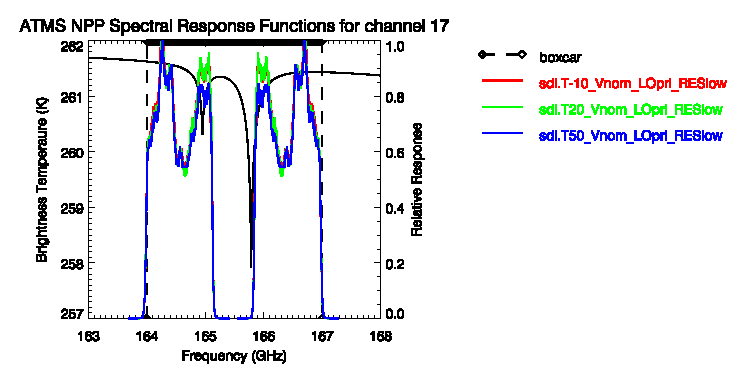
\includegraphics[bb=80 400 280 558,clip,scale=0.85]{graphics/srf/Tset/atms_npp.ch17.osrf.eps} &
    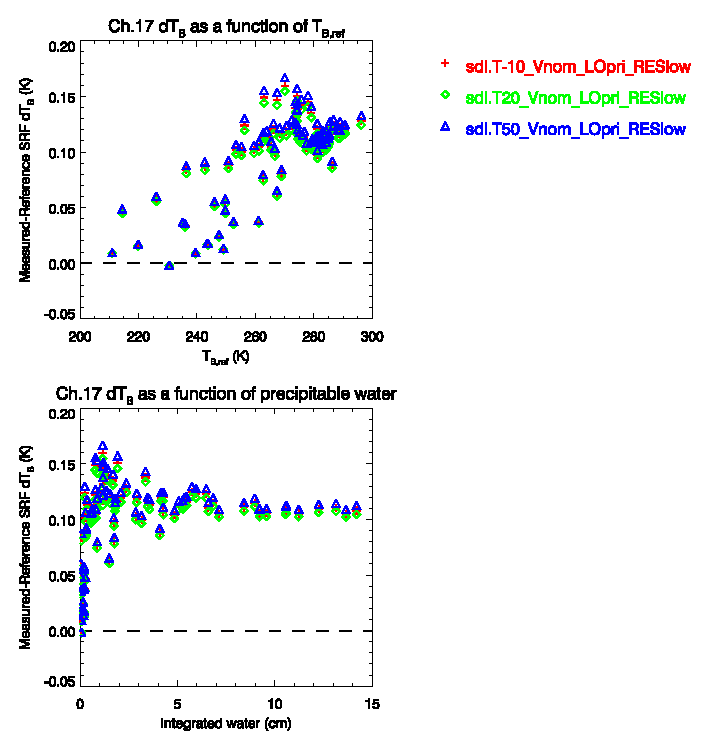
\includegraphics[bb=85 400 260 558,clip,scale=0.85]{graphics/dtb/Tset/e1.0_r0.0/atms_npp.ch17.dTb.eps} & 
    \includegraphics[bb=85 400 290 558,clip,scale=0.85]{graphics/dtb/Tset/e0.6_r0.4/atms_npp.ch17.dTb.eps} 
  \end{tabular} \\
  % the hand-crafted legend
  \setlength{\unitlength}{1cm}
  \begin{picture}(8.0,1.0)
    \thicklines
    \color{red}
    \put(0.0,0.5){\line(1,0){1}}
    \put(1.2,0.35){\sffamily \textbf{+}\quad -10\textdegree{}C}
    \color{green}
    \put(3.0,0.5){\line(1,0){1}}
    \put(4.2,0.35){\sffamily {\Large$\diamond$}\quad 20\textdegree{}C}
    \color{blue}
    \put(6.0,0.5){\line(1,0){1}}
    \put(7.2,0.35){\sffamily $\bigtriangleup$\quad 50\textdegree{}C}
  \end{picture}
  \caption{Channel 17 NPP ATMS \textbf{(a)} SRF data digitized from plots in the ATMS PFM Calibration Data Book\cite{ATMS_PFM_CalLog} with the corresponding boxcar response based on table \ref{tab:atms_fo_sb_and_df}. A representative brightness temperature spectrum is also shown. \textbf{(b)} Difference in the MonoRTM-derived brightness temperatures, using unity surface emissivity, as a function of the boxcar SRF $T_B$ for nominal bias voltage and three baseplate temperatures (-10, 20, and 50\textdegree{}C). \textbf{(c)} Same as (b), but for surface emissivity and reflectivity of 0.6 and 0.4 respectively. }
  \label{fig:atms_npp.Tset.ch17}
\end{figure}

\begin{figure}[H]
  \centering
  \begin{tabular}{c c c}
    \textsf{\textbf{(a)} SRFs} &
    \textsf{\textbf{(b)} $\Delta T_B$ $(\epsilon_s = 1.0)$} &
    \textsf{\textbf{(c)} $\Delta T_B$ $(\epsilon_s = 0.6)$} \\
    \includegraphics[bb=80 400 280 558,clip,scale=0.85]{graphics/srf/Tset/atms_npp.ch18.osrf.eps} &
    \includegraphics[bb=85 400 260 558,clip,scale=0.85]{graphics/dtb/Tset/e1.0_r0.0/atms_npp.ch18.dTb.eps} & 
    \includegraphics[bb=85 400 290 558,clip,scale=0.85]{graphics/dtb/Tset/e0.6_r0.4/atms_npp.ch18.dTb.eps} 
  \end{tabular} \\
  % the hand-crafted legend
  \setlength{\unitlength}{1cm}
  \begin{picture}(8.0,1.0)
    \thicklines
    \color{red}
    \put(0.0,0.5){\line(1,0){1}}
    \put(1.2,0.35){\sffamily \textbf{+}\quad -10\textdegree{}C}
    \color{green}
    \put(3.0,0.5){\line(1,0){1}}
    \put(4.2,0.35){\sffamily {\Large$\diamond$}\quad 20\textdegree{}C}
    \color{blue}
    \put(6.0,0.5){\line(1,0){1}}
    \put(7.2,0.35){\sffamily $\bigtriangleup$\quad 50\textdegree{}C}
  \end{picture}
  \caption{Channel 18 NPP ATMS \textbf{(a)} SRF data digitized from plots in the ATMS PFM Calibration Data Book\cite{ATMS_PFM_CalLog} with the corresponding boxcar response based on table \ref{tab:atms_fo_sb_and_df}. A representative brightness temperature spectrum is also shown. \textbf{(b)} Difference in the MonoRTM-derived brightness temperatures, using unity surface emissivity, as a function of the boxcar SRF $T_B$ for nominal bias voltage and three baseplate temperatures (-10, 20, and 50\textdegree{}C). \textbf{(c)} Same as (b), but for surface emissivity and reflectivity of 0.6 and 0.4 respectively. }
  \label{fig:atms_npp.Tset.ch18}
\end{figure}

\begin{figure}[H]
  \centering
  \begin{tabular}{c c c}
    \textsf{\textbf{(a)} SRFs} &
    \textsf{\textbf{(b)} $\Delta T_B$ $(\epsilon_s = 1.0)$} &
    \textsf{\textbf{(c)} $\Delta T_B$ $(\epsilon_s = 0.6)$} \\
    \includegraphics[bb=80 400 280 558,clip,scale=0.85]{graphics/srf/Tset/atms_npp.ch19.osrf.eps} &
    \includegraphics[bb=85 400 260 558,clip,scale=0.85]{graphics/dtb/Tset/e1.0_r0.0/atms_npp.ch19.dTb.eps} & 
    \includegraphics[bb=85 400 290 558,clip,scale=0.85]{graphics/dtb/Tset/e0.6_r0.4/atms_npp.ch19.dTb.eps} 
  \end{tabular} \\
  % the hand-crafted legend
  \setlength{\unitlength}{1cm}
  \begin{picture}(8.0,1.0)
    \thicklines
    \color{red}
    \put(0.0,0.5){\line(1,0){1}}
    \put(1.2,0.35){\sffamily \textbf{+}\quad -10\textdegree{}C}
    \color{green}
    \put(3.0,0.5){\line(1,0){1}}
    \put(4.2,0.35){\sffamily {\Large$\diamond$}\quad 20\textdegree{}C}
    \color{blue}
    \put(6.0,0.5){\line(1,0){1}}
    \put(7.2,0.35){\sffamily $\bigtriangleup$\quad 50\textdegree{}C}
  \end{picture}
  \caption{Channel 19 NPP ATMS \textbf{(a)} SRF data digitized from plots in the ATMS PFM Calibration Data Book\cite{ATMS_PFM_CalLog} with the corresponding boxcar response based on table \ref{tab:atms_fo_sb_and_df}. A representative brightness temperature spectrum is also shown. \textbf{(b)} Difference in the MonoRTM-derived brightness temperatures, using unity surface emissivity, as a function of the boxcar SRF $T_B$ for nominal bias voltage and three baseplate temperatures (-10, 20, and 50\textdegree{}C). \textbf{(c)} Same as (b), but for surface emissivity and reflectivity of 0.6 and 0.4 respectively. }
  \label{fig:atms_npp.Tset.ch19}
\end{figure}

\begin{figure}[H]
  \centering
  \begin{tabular}{c c c}
    \textsf{\textbf{(a)} SRFs} &
    \textsf{\textbf{(b)} $\Delta T_B$ $(\epsilon_s = 1.0)$} &
    \textsf{\textbf{(c)} $\Delta T_B$ $(\epsilon_s = 0.6)$} \\
    \includegraphics[bb=80 400 280 558,clip,scale=0.85]{graphics/srf/Tset/atms_npp.ch20.osrf.eps} &
    \includegraphics[bb=85 400 260 558,clip,scale=0.85]{graphics/dtb/Tset/e1.0_r0.0/atms_npp.ch20.dTb.eps} & 
    \includegraphics[bb=85 400 290 558,clip,scale=0.85]{graphics/dtb/Tset/e0.6_r0.4/atms_npp.ch20.dTb.eps} 
  \end{tabular} \\
  % the hand-crafted legend
  \setlength{\unitlength}{1cm}
  \begin{picture}(8.0,1.0)
    \thicklines
    \color{red}
    \put(0.0,0.5){\line(1,0){1}}
    \put(1.2,0.35){\sffamily \textbf{+}\quad -10\textdegree{}C}
    \color{green}
    \put(3.0,0.5){\line(1,0){1}}
    \put(4.2,0.35){\sffamily {\Large$\diamond$}\quad 20\textdegree{}C}
    \color{blue}
    \put(6.0,0.5){\line(1,0){1}}
    \put(7.2,0.35){\sffamily $\bigtriangleup$\quad 50\textdegree{}C}
  \end{picture}
  \caption{Channel 20 NPP ATMS \textbf{(a)} SRF data digitized from plots in the ATMS PFM Calibration Data Book\cite{ATMS_PFM_CalLog} with the corresponding boxcar response based on table \ref{tab:atms_fo_sb_and_df}. A representative brightness temperature spectrum is also shown. \textbf{(b)} Difference in the MonoRTM-derived brightness temperatures, using unity surface emissivity, as a function of the boxcar SRF $T_B$ for nominal bias voltage and three baseplate temperatures (-10, 20, and 50\textdegree{}C). \textbf{(c)} Same as (b), but for surface emissivity and reflectivity of 0.6 and 0.4 respectively. }
  \label{fig:atms_npp.Tset.ch20}
\end{figure}

\begin{figure}[H]
  \centering
  \begin{tabular}{c c c}
    \textsf{\textbf{(a)} SRFs} &
    \textsf{\textbf{(b)} $\Delta T_B$ $(\epsilon_s = 1.0)$} &
    \textsf{\textbf{(c)} $\Delta T_B$ $(\epsilon_s = 0.6)$} \\
    \includegraphics[bb=80 400 280 558,clip,scale=0.85]{graphics/srf/Tset/atms_npp.ch21.osrf.eps} &
    \includegraphics[bb=85 400 260 558,clip,scale=0.85]{graphics/dtb/Tset/e1.0_r0.0/atms_npp.ch21.dTb.eps} & 
    \includegraphics[bb=85 400 290 558,clip,scale=0.85]{graphics/dtb/Tset/e0.6_r0.4/atms_npp.ch21.dTb.eps} 
  \end{tabular} \\
  % the hand-crafted legend
  \setlength{\unitlength}{1cm}
  \begin{picture}(8.0,1.0)
    \thicklines
    \color{red}
    \put(0.0,0.5){\line(1,0){1}}
    \put(1.2,0.35){\sffamily \textbf{+}\quad -10\textdegree{}C}
    \color{green}
    \put(3.0,0.5){\line(1,0){1}}
    \put(4.2,0.35){\sffamily {\Large$\diamond$}\quad 20\textdegree{}C}
    \color{blue}
    \put(6.0,0.5){\line(1,0){1}}
    \put(7.2,0.35){\sffamily $\bigtriangleup$\quad 50\textdegree{}C}
  \end{picture}
  \caption{Channel 21 NPP ATMS \textbf{(a)} SRF data digitized from plots in the ATMS PFM Calibration Data Book\cite{ATMS_PFM_CalLog} with the corresponding boxcar response based on table \ref{tab:atms_fo_sb_and_df}. A representative brightness temperature spectrum is also shown. \textbf{(b)} Difference in the MonoRTM-derived brightness temperatures, using unity surface emissivity, as a function of the boxcar SRF $T_B$ for nominal bias voltage and three baseplate temperatures (-10, 20, and 50\textdegree{}C). \textbf{(c)} Same as (b), but for surface emissivity and reflectivity of 0.6 and 0.4 respectively. }
  \label{fig:atms_npp.Tset.ch21}
\end{figure}

\begin{figure}[H]
  \centering
  \begin{tabular}{c c c}
    \textsf{\textbf{(a)} SRFs} &
    \textsf{\textbf{(b)} $\Delta T_B$ $(\epsilon_s = 1.0)$} &
    \textsf{\textbf{(c)} $\Delta T_B$ $(\epsilon_s = 0.6)$} \\
    \includegraphics[bb=80 400 280 558,clip,scale=0.85]{graphics/srf/Tset/atms_npp.ch22.osrf.eps} &
    \includegraphics[bb=85 400 260 558,clip,scale=0.85]{graphics/dtb/Tset/e1.0_r0.0/atms_npp.ch22.dTb.eps} & 
    \includegraphics[bb=85 400 290 558,clip,scale=0.85]{graphics/dtb/Tset/e0.6_r0.4/atms_npp.ch22.dTb.eps} 
  \end{tabular} \\
  % the hand-crafted legend
  \setlength{\unitlength}{1cm}
  \begin{picture}(8.0,1.0)
    \thicklines
    \color{red}
    \put(0.0,0.5){\line(1,0){1}}
    \put(1.2,0.35){\sffamily \textbf{+}\quad -10\textdegree{}C}
    \color{green}
    \put(3.0,0.5){\line(1,0){1}}
    \put(4.2,0.35){\sffamily {\Large$\diamond$}\quad 20\textdegree{}C}
    \color{blue}
    \put(6.0,0.5){\line(1,0){1}}
    \put(7.2,0.35){\sffamily $\bigtriangleup$\quad 50\textdegree{}C}
  \end{picture}
  \caption{Channel 22 NPP ATMS \textbf{(a)} SRF data digitized from plots in the ATMS PFM Calibration Data Book\cite{ATMS_PFM_CalLog} with the corresponding boxcar response based on table \ref{tab:atms_fo_sb_and_df}. A representative brightness temperature spectrum is also shown. \textbf{(b)} Difference in the MonoRTM-derived brightness temperatures, using unity surface emissivity, as a function of the boxcar SRF $T_B$ for nominal bias voltage and three baseplate temperatures (-10, 20, and 50\textdegree{}C). \textbf{(c)} Same as (b), but for surface emissivity and reflectivity of 0.6 and 0.4 respectively. }
  \label{fig:atms_npp.Tset.ch22}
\end{figure}

